\documentclass{article}

\usepackage[parfill]{parskip}
\usepackage{
  geometry,
  float,
  listings,
  xcolor,
  amssymb,
  fontspec,
  graphicx,
  hyperref,
}

\graphicspath{ {docs/imgs/} }

% To keep figures, listings, and tables rendered where they're put
% *** BEGIN ***
\let\origfigure\figure
\let\endorigfigure\endfigure
\renewenvironment{figure}[1][2] {
    \expandafter\origfigure\expandafter[H]
} {
    \endorigfigure
}

\AtBeginDocument{\floatplacement{codelisting}{H}}
\AtBeginDocument{\floatplacement{table}{H}}
% *** END ***

\geometry{
  top = 20mm,
  bottom = 20mm,
  left = 25mm,
  right = 25mm,
  paper = a4paper,
}

\setmainfont{Times New Roman}
\setmonofont{JetBrainsMono Nerd Font Mono}

\definecolor{codegreen}{rgb}{0,0.6,0}
\definecolor{codegray}{rgb}{0.5,0.5,0.5}
\definecolor{codepurple}{rgb}{0.58,0,0.82}
\definecolor{backcolour}{rgb}{0.95,0.95,0.92}

\lstset{% https://en.wikibooks.org/wiki/LaTeX/Source_Code_Listings
  basicstyle = \footnotesize\ttfamily,
  breakatwhitespace = true,
  breaklines = true,
  frame = single,
  firstnumber = 1,
  keepspaces = true,
  numbers = left,
  tabsize = 4,
  backgroundcolor=\color{backcolour},
  commentstyle=\color{codegray},
  keywordstyle=\color{orange},
  numberstyle=\tiny\color{codegray},
  stringstyle=\color{codegreen},
  basicstyle=\ttfamily\footnotesize,
}

% https://github.com/gilangardya/if2211-cryptarithmetic-solver/blob/master/doc/LaporanTucil1.pdf

\begin{document}
\begin{titlepage}
  \centering
  \vspace*{\stretch{2}}
  \Large Laporan Tugas Kecil I

  \large Dekripsi \textit{Cryptarithmetic} dengan \textit{Brute Force}

  \normalsize

  \vspace{\stretch{1}}

  
\includegraphics[scale=0.2]{logo-itb.png}

  \vspace{\stretch{1}}
  \begin{tabular}{lll}
    Nama  &: & Josep Marcello \\
    NIM &: & 13519164 \\
    Kelas &: & K-03 \\
    Dosen &: & Prof. Dwi Hendratmo Widyantoro \\
    Bahasa &: & C++ \\
  \end{tabular}

  \vspace{\stretch{2}}
  \large
  PROGRAM STUDI TEKNIK INFORMATIKA

  SEKOLAH TEKNIK ELEKTRO DAN INFORMATIKA

  INSTITUT TEKNOLOGI BANDUNG

  BANDUNG

  2021

  \vspace{\stretch{2}}
\end{titlepage}

\section{Algoritma \textit{Brute Force}}
\begin{enumerate}
  \item Proses dekripsi \textit{cryptarithmetic} dimulai dengan pembuatan
    himpunan/matriks berukuran $10! \times 10$ yang berisi kemungkinan
    permutasi himpunan yang terdiri dari 10 angka (0, 1, 2, \ldots, 9).
  \item Selanjutnya, untuk soal yang ingin didekripsi, dicari huruf-huruf
    uniknya.
  \item Kemudian, setiap huruf unik akan di-\textit{assign} sebuah nilai yang
    diambil dari setiap anggota himpunan dari matriks yang dibuat pada langkah
    1.

    Misalnya jika anggota himpunannya adalah [5, 2, 0, 3, 4, 1, 8, 9,
    7, 6] dan huruf uniknya terdiri dari [C, T, A], maka C = 5, T = 2, A = 0,
    dan anggota himpunan lainnya ``dibuang''\footnote{Algoritma ini bisa
    menyebabkan rekalkulasi (misalnya jika anggota himpunannya adalah [5, 2, 0,
    1, 3, 4, 6, 7, 8, 9], maka C~=~5, T =~2, A~=~0), tapi setelah pengujian,
    cara ini bisa menyebabkan perhitungan lebih cepat jika diberikan beberapa
    soal sekaligus.}.
  \item Selanjutnya, diperiksa ada atau tidak huruf depan \textit{operand} yang
    di-\textit{assign} ke angka 0.
    \begin{itemize}
      \item Jika ada, kembali ke langkah sebelumna dan pilih anggota himpunan
        lain, tetapi
      \item jika tidak ada, lanjutkan ke langkah selanjutnya.
    \end{itemize}
  \item Kemudian, setiap huruf pada setiap operand akan diganti dengan angka
    yang sudah di-\textit{assign}-kan ke huruf yang bersangkutan kemudian angka
    itu akan dijumlahkan ke suatu variabel.
  \item Hasil diubah ke dalam bentuk angka juga.
  \item Lalu, variabel yang menjumlahkan semua \textit{operand} angka
    pada langkah 5 diperiksa sudah sama dengan hasil yang diubah ke angka atau
    belum.
    \begin{itemize}
      \item Jika sama, lanjutkan ke langkah selanjutnya, tetapi
      \item jika tidak sama, kembali ke langkah 2 dengan memilih anggota
        himpunan yang lain.
    \end{itemize}
  \item Pada langkah ini, program sudah selesai bekerja jika semua soal sudah
    didekripsi, tetapi jika masih ada soal lagi, program akan kembali ke
    langkah 2.
\end{enumerate}

\section{\textit{Source Code} Program}
\begin{lstlisting}[caption = main.cpp, language = c++]
/* Nama     : Josep Marcello
 * NIM      : 13519164
 * Tanggal  : 20 Januari 2021
 */

#include <chrono> // itung waktu eksekusi
#include <utility> // pairs
#include <vector> // vector
#include <stdlib.h> // exit(), free(), malloc()
#include <sysexits.h> // exit codes
#include <stdio.h> // printf(), puts(), scanf()
#include <iostream> // string, cout
#include <unordered_map> // unordered_map
#include <fstream> // file ops

#define MAX_UNIQUE_LETTERS 10
#define debug1() puts("males belajar tapi...")
#define debug2() puts("pengen kaya")
#define debug3() puts("udah stres")
#define cel() puts("")

// *** DEKLARASI FUNGSI-FUNGSI ***

/**
 * Fungsi untuk membuat semua kemungkinan permutasi dari suatu vektor
 *
 * @tparam T tipe data yang disimpan pada vektor
 * @param vec vektor yang ingin dibuat permutasinya
 * @returns vektor yg berisi vektor-vektor hasil permutasi
 */
template <typename T>
std::vector<std::vector<T>> permutate_vec(std::vector<T> vec);

/**
 * Fungsi untuk menghasilkan enumerasi permutasi-permutasi yang mungkin dari
 * angka-angka dalam range [0..lim)
 *
 * Mis: lim = 2, maka output:
 * [[0,1], [1,0]]
 *
 * lim = 3:
 * [[0,1,2], [0,2,1], [1,0,2], [1,2,0], [2,0,1], [2,1,0]]
 *
 * @param lim batas atas angka
 */
std::vector<std::vector<int>> generate_permutated_numbers(int lim);

/**
 * Fungsi untuk mendekripsi Cryptarithmetic
 *
 * @param soal soal yang mau didekripsi
 * @param permutatedNumbers vektor berisi vektor-vektor kumpulan
 * permutasi-permutasi yang mungkin dari vektor angka [0..MAX_UNIQUE_LETTERS]
 * @returns sebuah pair berisi solusi benar dan jumlah kasus yang dikerjakan
 */
std::pair<std::vector<int>, int> decrypt_cryparithm(std::vector<std::string> soal, std::vector<std::vector<int>> permutatedNumbers);

/**
 * Fungsi untuk mendapatkan huruf-huruf unik dari soal
 *
 * @param soal soal yang ingin dicari huruf-huruf uniknya
 */
std::vector<char> unique_letters(std::vector<std::string> soal);

/**
 * Fungsi untuk menuliskan jawaban sesuai dengan spek
 *
 * @param soal vektor yang berisi soal yang ingin diprint, hasil parse parse_file()
 * @param answer jawaban dari soal yang ingin diprint, hasil decrypt_cryparithm()
 */
void print_answer(std::vector<std::string> soal, std::vector<int> answer);

/**
 * Fungsi untuk membaca file (sesuai format pada spek) lalu memisahkannya
 * berdasarkan soal
 *
 * @param *fileName string yang berisi nama file soal
 * @param *output vector dari vector yang menampung soal-soal (tiap elemen
 * adalah soal)
 */
void parse_file(char* fileName, std::vector<std::vector<std::string>>* output);

/**
 * Fungsi untuk menghapuskan whitespaces ('', '\t', '\n') dari awal C string
 *
 * @param *strToStrip pointer ke C string yang ingin di-strip
 * @returns std::string yang sudah dihapuskan whitespace-nya
 */
std::string strip_at_beginning(char* strToStrip);

// *** END ***

int main(int argc, char *argv[])
{
    /// Vektor untuk nyimpen semua soal
    std::vector<std::vector<std::string>> semuaSoal;

    if (argc == 1)
    {
        /*
        fprintnf(stderr, "Penggunaan: %s [nama file soal]\n", argv[0]);
        exit(EX_USAGE);
        */

        /// string berisi nama file soal
        char* namaFile;
        namaFile = (char *) malloc(128 * sizeof(char));

        printf("Masukkan nama file: ");
        scanf("%s", namaFile);
        getchar();
        parse_file(namaFile, &semuaSoal);
        free(namaFile);
    }
    else parse_file(argv[1], &semuaSoal);

    std::chrono::steady_clock sc;

    /// Vektor untuk menyimpan semua jawaban
    std::vector<std::vector<int>> answers(semuaSoal.size());

    /// awal perhitungan waktu semua soal
    auto start = sc.now();
    /// Vektor untuk menyimpan semua kemungkinan permutasi dari [0..9]
    std::vector<std::vector<int>> permutatedNumbers = generate_permutated_numbers(MAX_UNIQUE_LETTERS);
    /// akhir perhitungan waktu pembuatan permutasi list
    auto permEnd = sc.now();
    auto permTS = static_cast<std::chrono::duration<double>>(permEnd-start);
    printf("Waktu pembuatan semua kemungkinan permutasi adalah: %lf.\n\n", permTS.count());
    for (std::vector<std::vector<std::string>>::iterator it =
            semuaSoal.begin(); it != semuaSoal.end(); ++it)
    {
        /// awal hitungan waktu
        auto partialStart = sc.now();

        /// counter iterasi
        int i = it - semuaSoal.begin();
        /// jumlah kasus yg diuji
        int cases;

        // dekripsi dan tuliskan hasil
        std::pair<std::vector<int>, int> result = decrypt_cryparithm(*it, permutatedNumbers);
        answers[i] = result.first;
        cases = result.second;

        print_answer(*it, answers[i]);
        printf("\n");

        /// akhir hitungan waktu
        auto partialEnd = sc.now();
        auto partialTimeSpend = static_cast<std::chrono::duration<double>>(partialEnd-partialStart);
        printf("Soal ke-%d membutuhkan: %lf detik.\n", i+1, partialTimeSpend.count());
        printf("Jumlah kasus yang diuji adalah %d.\n\n", cases);
    }

    // akhir perhitungan waktu semua soal
    auto end = sc.now();
    auto timeSpend = static_cast<std::chrono::duration<double>>(end-start);

    printf("Total waktu permutasi, eksekusi dekripsi %lu soal, dan menuliskan output adalah %lf detik.\n",
            semuaSoal.size(), timeSpend.count());
}

template <typename T>
std::vector<std::vector<T>> permutate_vec(std::vector<T> vec)
{
    if (vec.size() == 0) return {{}};
    else if (vec.size() == 1) return {vec};
    else if (vec.size() == 2) return {vec, {vec[1], vec[0]}};

    /// vektor yang menampung hasil semua permutasi
    std::vector<std::vector<T>> newVec;
    /// elemen pertama vektor
    T first = vec[0];
    /// tail yang sudah dipermutasi
    std::vector<std::vector<T>> permutated = permutate_vec(std::vector<T>(vec.begin()+1, vec.end()));

    // tambahin first ke setiap hasil permutasi tail

    /// elemen dari permutated (tail yang sudah dipermutasi)
    for (std::vector<T> p: permutated)
    {
        for (size_t i = 0; i < p.size() + 1; ++i)
        {
            /// vektor yang akan dipush ke newVec
            std::vector<T> toBePushed(p.begin(), p.begin()+i);
            toBePushed.push_back(first);
            toBePushed.insert(toBePushed.end(), p.begin()+i, p.end());

            newVec.push_back(toBePushed);
        }
    }

    return newVec;
}

std::vector<std::vector<int>> generate_permutated_numbers(int lim)
{

    /// vektor untuk menyimpan angka-angka pada vektor
    std::vector<int> numbers(lim);
    for (int i = 0; i < lim; ++i)
        numbers[i] = i;

    std::vector<std::vector<int>> hasil = permutate_vec(numbers);

    return hasil;
}

std::pair<std::vector<int>, int> decrypt_cryparithm(std::vector<std::string> soal, std::vector<std::vector<int>> permutatedNumbers)
{
    // proses perisapan dan inisialisasi

    /// vektor untuk menyimpan huruf-huruf unik
    std::vector<char> letters = unique_letters(soal);
    /// vektor untuk menyimpan huruf pertama dari tiap operand
    std::vector<char> firstLetters(soal.size());
    /// unordered_map yang memetakan huruf ke angka
    std::unordered_map<char, int> numberFromLetter;
    /// counter jumlah kasus
    int cases = 0;

    // bikin vektor huruf pertama
    for (std::vector<std::string>::iterator it = soal.begin();
            it != soal.end();
            ++it)
        firstLetters[it - soal.begin()] = ((*it)[0]);

    // probably not needed, but wut teh hecc
    if (letters.size() > MAX_UNIQUE_LETTERS)
    {
        std::cerr << "Banyak huruf berbeda (unik) maksimum adalah "
                << MAX_UNIQUE_LETTERS << '.';
        exit(EX_DATAERR);
    }

    /// vektor u/ nampung operands yg udh diubah ke dalam bentuk bilangan
    std::vector<int> operandInNumbers(soal.size());

    // proses dekripsi

    /// numbers vektor yang berisi angka [0..9] yang sudah dipermutasi
    for (std::vector<int> numbers: permutatedNumbers)
    {
        operandInNumbers.clear();
        // map huruf ke angka
        for (size_t i = 0; i < letters.size(); ++i)
            numberFromLetter[letters[i]] = numbers[i];

        // periksa huruf pertama ada yg bernilai 0 atau ngga

        /// Penanda apakah loop perlu dilanjutkan atau tidak
        bool stopThyLoop = false;
        for (char c: firstLetters) stopThyLoop = numberFromLetter[c] == 0;

        if (stopThyLoop) continue;

        /// variabel untuk menyimpan sum dari semua operand
        int sum = 0,
        /// variabel untuk menyimmpan sum 'yang seharusnya'
            realSum = 0;

        // ubah operand-operand menjadi angka
        for (size_t i = 0; i < soal.size(); ++i)
        {
            int curNum = 0;
            for (size_t j = 0; j < soal[i].size(); ++j)
                curNum = curNum*10 + numberFromLetter[soal[i][j]];

            if (i != soal.size()-1)
                sum += curNum;
            else
                realSum = curNum;

            operandInNumbers.push_back(curNum);
        }

        if (sum == realSum) break;
        else cases++;
    }

    return std::make_pair(operandInNumbers, cases);
}

std::vector<char> unique_letters(std::vector<std::string> soal)
{
    /// vector untuk nyimpen huruf-huruf unik
    std::vector<char> letters;

    /// array untuk nandain huruf apa aja yg udah dipake
    bool areLettersUsed[] = {
        false, false, false, false, false, false,
        false, false, false, false, false, false,
        false, false, false, false, false, false,
        false, false, false, false, false, false,
        false, false, false, false, false, false
    };

    for (std::string operand: soal)
    {
        for (char c: operand)
        {
            if (!areLettersUsed[c - 'A'])
            {
                letters.push_back(c);
                areLettersUsed[c - 'A'] = true;
            }
        }
    }

    return letters;
}

void print_answer(std::vector<std::string> soal, std::vector<int> answer)
{
    size_t longest = 0;
    for (std::string operand: soal)
        if (longest < operand.size()) longest = operand.size();


    for (size_t i = 0; i < soal.size()-2; ++i)
    {
        for (size_t j = 0; j < longest - soal[i].size(); ++j) // ngasih spasi
            std::cout << " ";
        std::cout << soal[i] << '\n';
    }
    for (size_t j = 0; j < longest - soal[soal.size()-2].size(); ++j) // ngasih spasi
        std::cout << " ";
    std::cout << soal[soal.size()-2] << " +\n";

    for (size_t i = 0; i < longest+2; ++i)
        std::cout << '-';
    std::cout << '\n';

    for (size_t j = 0; j < longest - soal[soal.size()-1].size(); ++j) // ngasih spasi
        std::cout << " ";
    std::cout << soal[soal.size()-1] << '\n';

    std::cout << '\n';
    std::cout << '\n';

    for (size_t i = 0; i < answer.size()-2; ++i)
    {
        for (size_t j = 0; j < longest - std::to_string(answer[i]).size(); ++j) // ngasih spasi
            std::cout << " ";
        std::cout << answer[i] << '\n';
    }

    for (size_t j = 0; j < longest - std::to_string(answer[answer.size()-2]).size(); ++j) // ngasih spasi
        std::cout << " ";
    std::cout << answer[answer.size()-2] << " +\n";

    for (size_t i = 0; i < longest+2; ++i)
        std::cout << '-';
    std::cout << '\n';

    for (size_t j = 0; j < longest - soal[soal.size()-1].size(); ++j) // ngasih spasi
        std::cout << " ";
    std::cout << answer[answer.size()-1] << '\n';
}

std::string strip_at_beginning(char* strToStrip)
{
    while ((*strToStrip == ' ' || *strToStrip == '\t' || *strToStrip == '\n')
            && (*strToStrip != '\0')) strToStrip++;

    return strToStrip;
}

void parse_file(char* fileName, std::vector<std::vector<std::string>>* output)
{
    /// variabel untuk menyimpan file
    std::fstream input;
    input.open(fileName, std::ios::in);

    if (input.is_open())
    {
        /// menyimpan baris dari file yang lagi mau diparse
        std::string line;

        while(getline(input, line))
        {
            /// vektor buat nyimpen operand-operand yang dibaca
            std::vector<std::string> operands;
            /// buat ngecek masih ngerjain ngeparse soal atau bukan
            bool isMasihParseSoal = true;
            /// buat ngecek udah operand terakhir atau belum
            bool isReadingLastOperand = false;

            do
            {
                /// operand yang lagi dibaca, sesudah di-strip di depan
                std::string operand = strip_at_beginning(&(line[0])).c_str();

                if (isReadingLastOperand)
                {
                    isMasihParseSoal = false;
                    operands.push_back(operand);
                }
                else if (operand.empty() || operand[0] == '-')
                {
                    isReadingLastOperand = operand[0] == '-';
                    continue;
                }
                else if (*(operand.end()-1) == '+')
                {
                    operand.resize(operand.size()-1);
                    operands.push_back(operand);
                }
                else operands.push_back(operand);
            } while(isMasihParseSoal && getline(input, line));

            output->push_back(operands);
        }

        input.close();
    }
    else
    {
        std::cerr << "Gagal membuka file " << fileName << ".\n";
        exit(EX_NOINPUT);
    }
}
\end{lstlisting}

\section{Hasil Pengujian}

\subsection{\textit{Input}}
\begin{figure}
  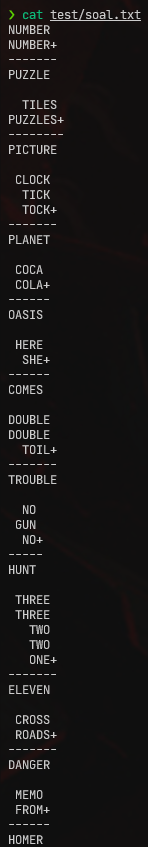
\includegraphics{stima-ss-3.png}
  \caption{Masukan program (10 soal)}
\end{figure}

\subsection{\textit{Output}}
\begin{figure}
  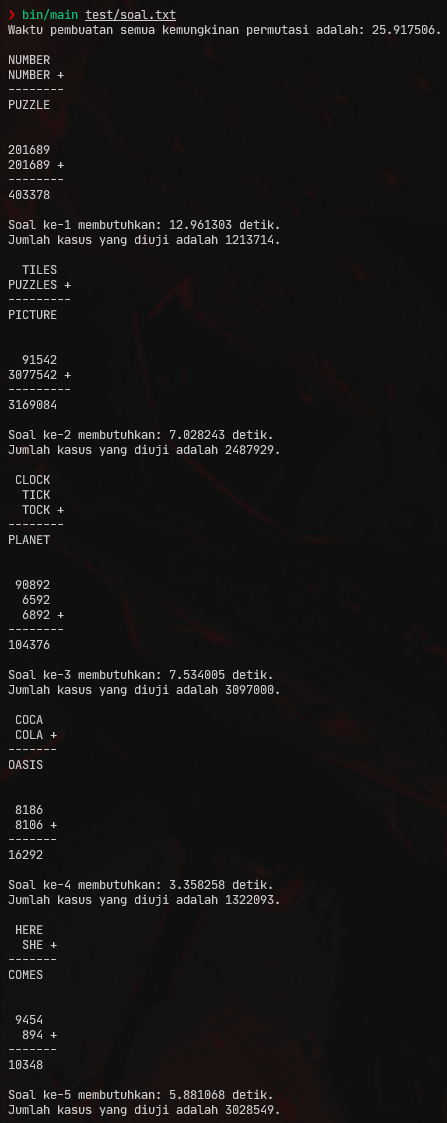
\includegraphics{stima-ss-1.png}
  \caption{Luaran program dekripsi untuk bagian permutasi dan soal 1 sampai 5}
\end{figure}
\begin{figure}
  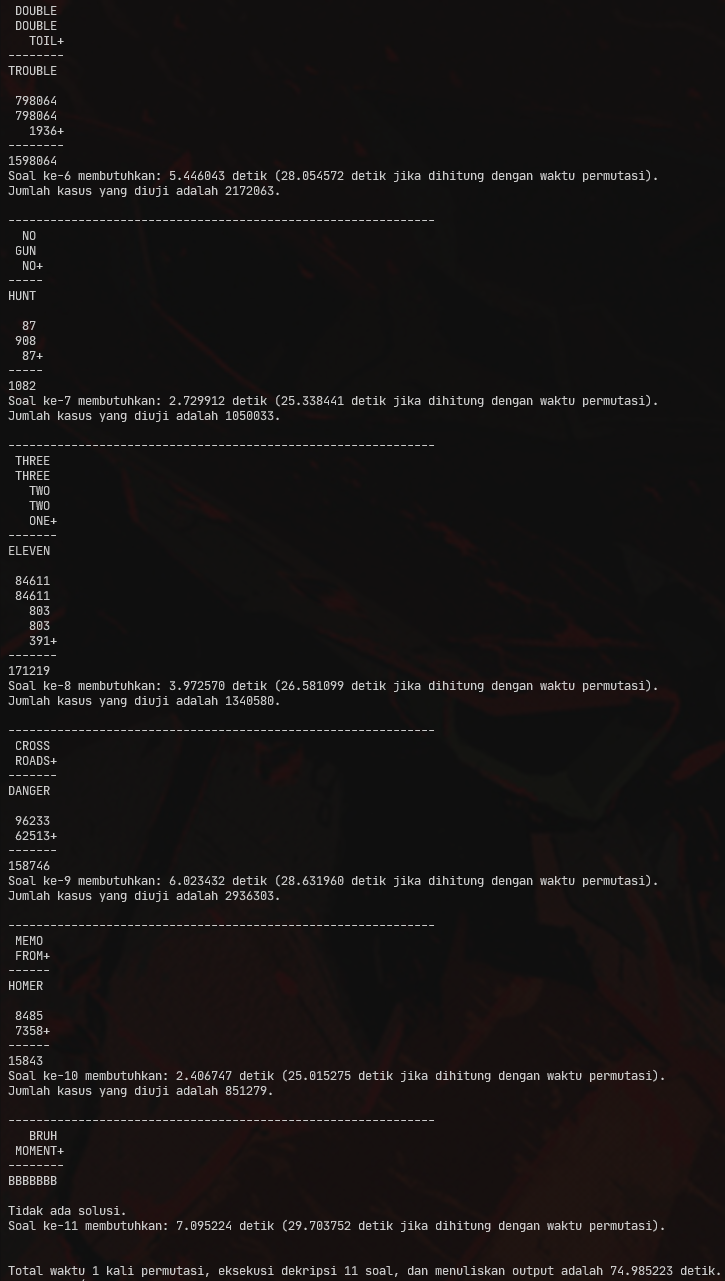
\includegraphics[scale = 0.9]{stima-ss-2.png}
  \caption{Luaran program dekripsi untuk soal 6 sampai 10}
\end{figure}

\subsection{Tabel Penilaian}
\begin{table}
  \begin{center}
    \begin{tabular}{|p{7cm} | l | l|}
      \hline
      Poin & Ya & Tidak \\
      \hline
      1. Program berhasil dikompilasi tanpa kesalahan (no syntax error) & \checkmark & \\
      \hline
      2. Program berhasil \textit{running} & \checkmark & \\
      \hline
      3. Program dapat membaca file masukan dan menuliskan luaran & \checkmark & \\
      \hline
      4. Solusi \textit{cryptarithmetic} hanya benar untuk persoalan \textit{cryptarithmetic} dengan dua buah \textit{operand} & & \checkmark \\
      \hline
      5. Solusi \textit{cryptarithmetic} benar untuk persoalan \textit{cryptarithmetic} untuk lebih dari dua buah \textit{operand} & \checkmark & \\
      \hline
    \end{tabular}
  \end{center}
\end{table}

\section*{\textit{Link} ke \textit{repository} Github}
\href{https://github.com/jspmarc/Tucil-1-Stima}{https://github.com/jspmarc/Tucil-1-Stima}

\end{document}
